\documentclass[12pt]{article}
\newcommand\tab[1][0.5cm]{\hspace*{#1}}
\usepackage[utf8]{inputenc}
\usepackage{listings}
\usepackage{hyperref}
\usepackage{color}
\pagenumbering{gobble}
\usepackage{changepage}
\usepackage{titletoc}
\usepackage{titlesec}
\usepackage{multicol}
\usepackage{graphicx}

\usepackage{makecell}

\definecolor{codegreen}{rgb}{0,0.6,0}
\definecolor{codegray}{rgb}{0.5,0.5,0.5}
\definecolor{codepurple}{rgb}{0.58,0,0.82}
\definecolor{backcolour}{rgb}{0.95,0.95,0.92}

\hypersetup{
	colorlinks,
	citecolor=black,
	filecolor=black,
	linkcolor=black,
	urlcolor=black
}

\lstdefinestyle{mystyle}{
	backgroundcolor=\color{backcolour},   
	commentstyle=\color{codegreen},
	keywordstyle=\color{magenta},
	numberstyle=\tiny\color{codegray},
	stringstyle=\color{codepurple},
	basicstyle=\footnotesize\ttfamily,
	breakatwhitespace=false,         
	breaklines=true,                 
	captionpos=b,                    
	keepspaces=true,                 
	numbers=left,                    
	numbersep=5pt,                  
	showspaces=false,                
	showstringspaces=false,
	showtabs=false,                  
	tabsize=3
}

\lstset{style=mystyle}

\newcommand{\titledate}[2][2.5in]{%
	\noindent%
	\begin{tabular}{@{}p{#1}@{}}
		\\ \hline \\[-.75\normalbaselineskip]
		#2
	\end{tabular} \hspace{1in}
	\begin{tabular}{@{}p{#1}@{}}
		\\ \hline \\[-.75\normalbaselineskip]
		Date
	\end{tabular}
}

\titleformat{\section}{\normalfont\Large\bfseries}{}{0pt}{}

% for forcing tables to fit
\usepackage{changepage}

\begin{document}
	

\begin{titlepage}
	
\author{Eric Pereira}
\date{Septemer 08\textsuperscript{th}, 2019}
\title{CSE4501 -- Vulnerability Research:\\Lab 1}

\maketitle

\end{titlepage}

\titlecontents{section}[0em]
{\vskip 0.5ex}%
{\scshape}% numbered sections formattin
{\itshape}% unnumbered sections formatting
{}%

\tableofcontents

\newpage \pagenumbering{arabic}

%%%%%%%%%%%%%%%%%%%%%%%%%%%%%%%%%%%%%%%%%%%%%%%%%%%%%%%%%%%%%%%%%%%%%%%%%%%%%%%%%%
%                                                                                %
%                                   Problem 1                                    %
%                                                                                %
%%%%%%%%%%%%%%%%%%%%%%%%%%%%%%%%%%%%%%%%%%%%%%%%%%%%%%%%%%%%%%%%%%%%%%%%%%%%%%%%%%

\section{Problem 1}
\tab Compile the below program; open in disassembler and compare source code with assembled
instructions. Explain why the binary is ~8K when it only has an empty function? Is there an
oddity with the instructions assembled? Do you see that in the machine code directly?
\begin{lstlisting}[language=C]
void main(){
}
\end{lstlisting}
\textbf{\\Solution:\\} 

The binary is quite large, at a total of about 7.2kB on my VM, whereas the C code for is about 15 bytes. I decided I would start by not
immediately looking at the binaries and just checking out a few things in the file itself. I did this by running ``\texttt{nm problem1}".

What I got was quite a lot more than I expected, I got a large list of responses, it looks like there is actually quite a bit going on. I
had quite a lot of stuff going on when I also ran ``\texttt{strings problem1}", so I decided to give it a look. It turns out that there is
in fact quite a lot going on. 

It looks like there is quite a lot happening at the start of the compiled c file, it clears the stack immediately in the start. It appears 
that, although there is nothing really going on in the program, there is quite a lot of setup in order to create a clean c file in order to
execute the commands you want to do. I suppose such a large initial set of instructions for cleanup is a large part of the reason why the 
compiled is so big. 


\newpage

%%%%%%%%%%%%%%%%%%%%%%%%%%%%%%%%%%%%%%%%%%%%%%%%%%%%%%%%%%%%%%%%%%%%%%%%%%%%%%%%%%
%                                                                                %
%                                   Problem 2                                    %
%                                                                                %
%%%%%%%%%%%%%%%%%%%%%%%%%%%%%%%%%%%%%%%%%%%%%%%%%%%%%%%%%%%%%%%%%%%%%%%%%%%%%%%%%%
\section{Problem 2}
\tab Compile the below program; open in disassembler and compare source code with assembled
instructions. What do you see on the stack frame? How is it different than Problem 1?
\begin{lstlisting}[language=C]
int main(){
	return 2;
}
\end{lstlisting}
\textbf{\\Solution:\\}

There is one major difference in the main function, that difference being that instead of a \texttt{nop} command, the value \texttt{2} is
pushed into \texttt{EAX} and the popped from the stack. Essentially it behaves nearly similarly, however it pushes 2 onto the stack when running, whereas problem has a ``\texttt{nop}" in its place instead. 

One thing I noticed is that problem 2 executable file is exactly the same size as problem 1 executable. So the only difference I noticed is
that one line where it pushes 2 onto the stack instead of a ``\texttt{nop}", and because the file size is identical I assume that that is
probably the only difference inside the actual executable, very interesting.  


%%%%%%%%%%%%%%%%%%%%%%%%%%%%%%%%%%%%%%%%%%%%%%%%%%%%%%%%%%%%%%%%%%%%%%%%%%%%%%%%%%
%                                                                                %
%                                   Problem 3                                    %
%                                                                                %
%%%%%%%%%%%%%%%%%%%%%%%%%%%%%%%%%%%%%%%%%%%%%%%%%%%%%%%%%%%%%%%%%%%%%%%%%%%%%%%%%%
\newpage
\section{Problem 3}
\tab Compile the below program; open in disassembler and compare source code with assembled
instructions. Specifically examine how the order of the stack is generated, do you see a
difference? You will need to use a debugger for this exercise.
\begin{lstlisting}[language=C]
#include <stdlib.h>
#include <stdio.h>

#define __cdecl __attribute__((__cdecl__))
#define __stdcall __attribute__((__stdcall__))
#define __fastcall __attribute__((__fastcall__))

int __cdecl print1(char string[]){
	printf("%s", string);
	return 0;
}

int __stdcall print2(char string[]){
	printf("%s", string);
	return 0;
}

int __fastcall print3(char string[]){
	printf("%s", string);
	return 0;
}

int main(int argc, char **argv){
	print1("First Call is cdecl.\n");
	print2("Second Call is stdcall.\n");
	print3("Third Call is fastcall.\n");
	return 0;
}
\end{lstlisting}
\textbf{\\Solution:\\} 

Each individual print functions works ever so slightly differently, they mostly look identical though. 

In fact, ``\texttt{\_\_cdecl}" and ``\texttt{\_\_stdcall}" are almost identical, there is one slight difference. The slight difference has
to do with stack cleanup. In ``\texttt{\_\_stdcall}" the stack is cleaned up by the actual ``\texttt{\_\_stdcall}" itself, whereas in the
``\texttt{\_\_cdecl}" it is not. This is reflected in the binaries:
\begin{multicols}{2}
	\begin{center}
		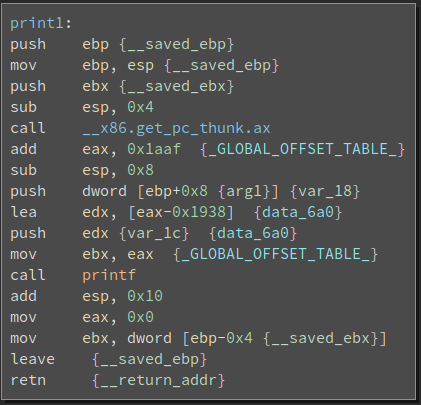
\includegraphics[width=\linewidth]{print1.png}
		Figure 1: print1 with ``\texttt{\_\_cdecl}"
		
	\end{center}

	\columnbreak

	\begin{center}
		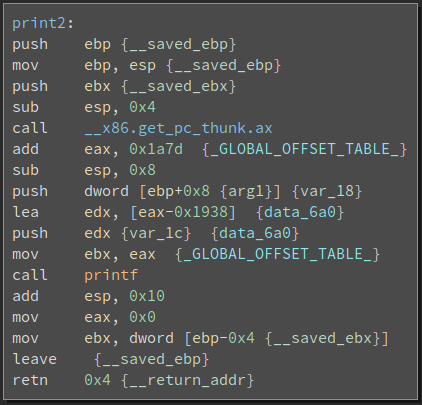
\includegraphics[width=\linewidth]{print2.png}
		Figure 2: print2 with ``\texttt{\_\_stdcall}"
	\end{center}
\end{multicols}

The difference is very clear when observing the last line, very interesting. Now there is also a difference with the print3 using the
``\texttt{\_\_fastcall}". Let's take a look at that. 

\begin{center}
	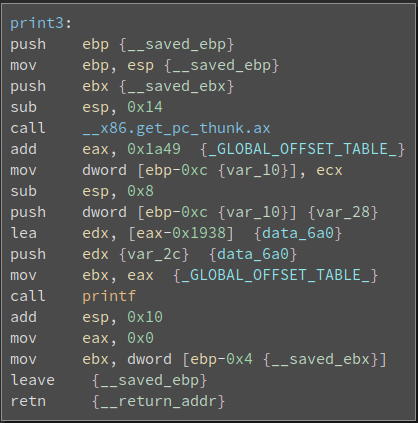
\includegraphics[scale=0.65]{print3.png} \\
	Figure 3: print3 with ``\texttt{\_\_fastcall}"
\end{center}

``\texttt{\_\_fastcall}" seems to use more of the registers initially, as when it moves the value of \texttt{ecx} which makes it a bit
different. Also, where in the ``\texttt{\_\_cdecl}" and ``\texttt{\_\_stdcall}" it will \texttt{sub esp, 0x4} in the \texttt{\_\_fastcall's
print3} it is instead \texttt{sub esp, 0x14}, very interesting. 



\newpage

%%%%%%%%%%%%%%%%%%%%%%%%%%%%%%%%%%%%%%%%%%%%%%%%%%%%%%%%%%%%%%%%%%%%%%%%%%%%%%%%%%
%                                                                                %
%                                   Problem 4                                    %
%                                                                                %
%%%%%%%%%%%%%%%%%%%%%%%%%%%%%%%%%%%%%%%%%%%%%%%%%%%%%%%%%%%%%%%%%%%%%%%%%%%%%%%%%%
\section{Problem 4}
\tab Compile the below program; open in disassembler and compare source code with assembled
instructions. Is the program using CDECL or STDCALL calling convention? Can you find the
string in the binary? Where is the string on the heap? You will need to use a debugger for this
exercise.

\begin{lstlisting}[language=C]
#include <stdio.h>
#include <string.h>
#include <stdlib.h>

char msg[] = "Chris is the coolest";

int main(){
int len = strlen(msg);

char *msgptr;
msgptr = malloc(len*sizeof(char)+1);
memcpy(msgptr, msg, len*sizeof(char)+1);
printf("Msg: %s\n", msgptr);

return 0;
}
\end{lstlisting}
\textbf{\\Solution:\\} 

This one is pretty easy, to put simply without having to show the binary it uses \texttt{\_\_cdecl}. You can tell it uses \texttt{\_\_cdecl}
because the function itself does not handle stack cleaning, as \texttt{\_\_stdcall} would, instead the parent function handles it. This 
indication makes it very easy to point out that this is \texttt{\_\_cdecl}


\newpage

%%%%%%%%%%%%%%%%%%%%%%%%%%%%%%%%%%%%%%%%%%%%%%%%%%%%%%%%%%%%%%%%%%%%%%%%%%%%%%%%%%
%                                                                                %
%                                   Problem 5                                    %
%                                                                                %
%%%%%%%%%%%%%%%%%%%%%%%%%%%%%%%%%%%%%%%%%%%%%%%%%%%%%%%%%%%%%%%%%%%%%%%%%%%%%%%%%%
\section{Problem 5}
\tab Analyze the crackme named “crackme” and solve. The crackme can be found in the files share
on canvas under Lab1
\\ \\
\textbf{Solution:} \\ 

This was quite frankly a very easy binary to review.

Before running the code I did a few things. The first thing I did was run \texttt{file crackme}. In a return I got an non-stripped,
dynamically-linked ELF-32 bit executable. I then ran \texttt{nm crackme}, which then didn't show me anything very interesting, at least not
interesting enough for me to pay attention. I lastly ran \texttt{strings crackme} and found something incredibly interesting.

What I found was a string ``\texttt{Enter Password:}", which means that this code will have me inputting some sort of password. 
Conveniently under that I found the totally not suspicious string ``\texttt{47ghf6fh37fbgbgj}''. Very interesting. 

At this point I decided I would run the code. I got the expected ``\texttt{Enter Password:}". Upon this I entered the string I found,
``\texttt{47ghf6fh37fbgbgj}'', and got the output: \\ 
\textbf{-[ Good, You're ready to begin linux reversing ]-}.

Well, I suppose I got quite lucky, I didn't even have to review the binary, and the problem did'nt even tell me I had to review the
binary, it said 'analyze the crackme'. I suppose my work is done then. \\
.......................................................................................................................

However, I still did want to analyze the binary so I did that anyways, I started by opening up the crackme in Binary Ninja. It was very easy
to crack when viewing the image actually, this is what it looked like:

\begin{center}
	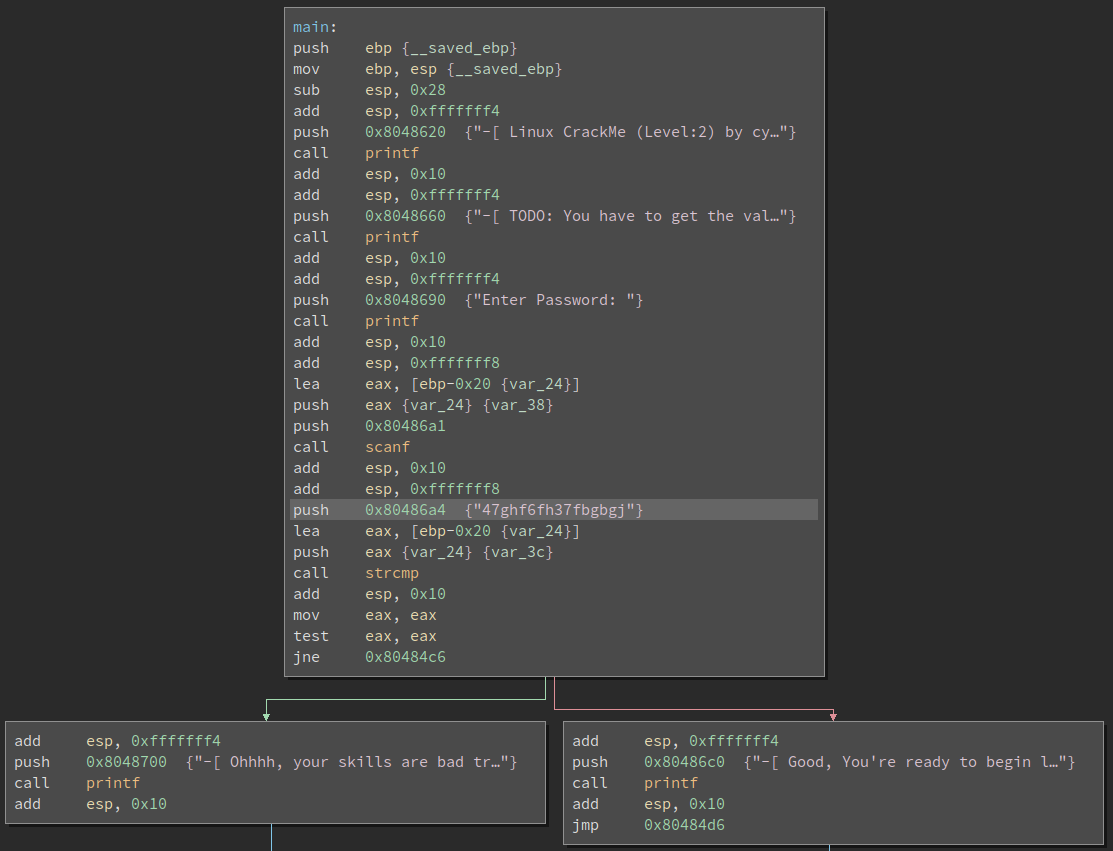
\includegraphics[scale=.5]{problem5.png}
\end{center}

It's obvious from here you push a specific string, and run a string compare from user input to this string. if it matches you get a message
that tells you that you are ready to begin linux reversing, else you get a message that tells you that you are a loser. 




\newpage

%%%%%%%%%%%%%%%%%%%%%%%%%%%%%%%%%%%%%%%%%%%%%%%%%%%%%%%%%%%%%%%%%%%%%%%%%%%%%%%%%%
%                                                                                %
%                                   Problem 6                                    %
%                                                                                %
%%%%%%%%%%%%%%%%%%%%%%%%%%%%%%%%%%%%%%%%%%%%%%%%%%%%%%%%%%%%%%%%%%%%%%%%%%%%%%%%%%
\section{Problem 6}
Extra Credit (0 pts, begin accumulating your L33T status) \\

Analyze the crackme “save\_scooby” and create a keygen. The crackme can be found in the
files share on canvas under Lab1
\\ \\
\textbf{Solution:\\} 

Extra credit with 0 points attached just seems like extra work, but extra work I shall do. 

Primarily, I first tried to see the file type, which was surprisingly an ELF-64 bit. This means that I am unable to use Binary Ninja,
because the trial version only allows for taking apart 32 bit binaries. Upsetting. 

I then tried to see if I could ``Cheat" by simply analyzing the strings like I did in the last problem, and, in a way, I sort of did fudge up
a correct answer.

Now, I was looking at Ida64 binary for a bit and to be honest I was a bit annoyed from reading everything, everything was in the main, I 
might as well look at it in C. I threw everything into Ghidra, and just had Ghidra do all the work of dissassembling to something in C. Ahh,
much more legible Now, what I noticed is that one of the local variables saves the \texttt{cwd} and edits it. It stores it as
the same thing initially, except it replaces all the `/' with `\$'. If the character in the \texttt{cwd} is not a `\' then it is turned into 
another character via an algorithm represented by the algorithm here:

\begin{center}
	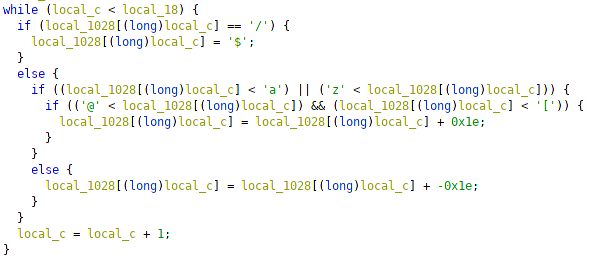
\includegraphics[scale=.92]{algorithm6.png}
\end{center}

After this the program asks for input. Now the expected input is the string that compares the obfuscated directory you are in, however I 
noticed that it is not necessarily a full string compare, it just compares the strings that are similar, so if you are in the home directory
you can just put in the string `\$' and it works. So, because I am lazy, and I don't feel like obfuscating, I took the easy way out. Here is
the code example to show how this may work:

\begin{center}
	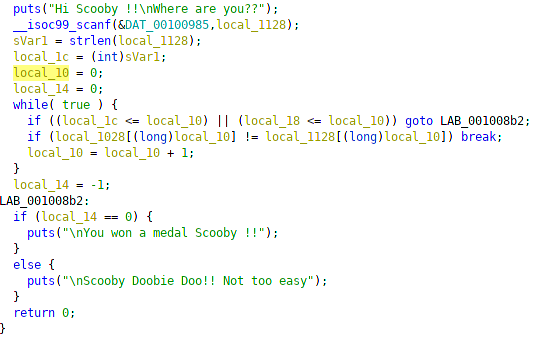
\includegraphics[scale=.96]{problem6.png}
\end{center}



\end{document}
